\chapter{Experimental Methods}
%Os experimentos são descritos aqui. 
In order to compare experimental results with the theoretical prevision we must measured two parameters in the Eq.\ref{eq:taxa_ir_broad} and \ref{eq:taxa_vis_broad}. First we need to characterize the visible mode by measure the losses $\kappa^(i)_3$ and $\kappa^(e)_3$; we have apply two different complementary techniques for that. The second important parameter is the Coupling terms $B_1$ and $B_3$; the challenge lays in the calculation of the overlap integral, as defined in Eq~\ref{eq:overlap_j3}, since it is necessary to identify the optical modes related in the THG. With this values in hand, we must be able to compare the theoretical and experimental results. 

However, first of all, the main experiment in this dissertation is the generation of third harmonic in optical microcavities. Lets star by there. This Chapter present a scientific description of the experiments, meanwhile a technical overview is presented in the Appendix~\ref{app:experiment}

\section{Third Harmonic Generation in Optical Microcavities}

The experiment is done with a setup quite similar to the one used in the optical characterization of infrared modes, show in Fig~\subref{fig:exp_mode_charac}{a}, with the inclusion of a wave modulator, a Erbium Doped Fiber Amplifier and a free space setup in the output to split the infrared (which was high powered) from the third harmonic.
\begin{figure}[h!]
    \centering
    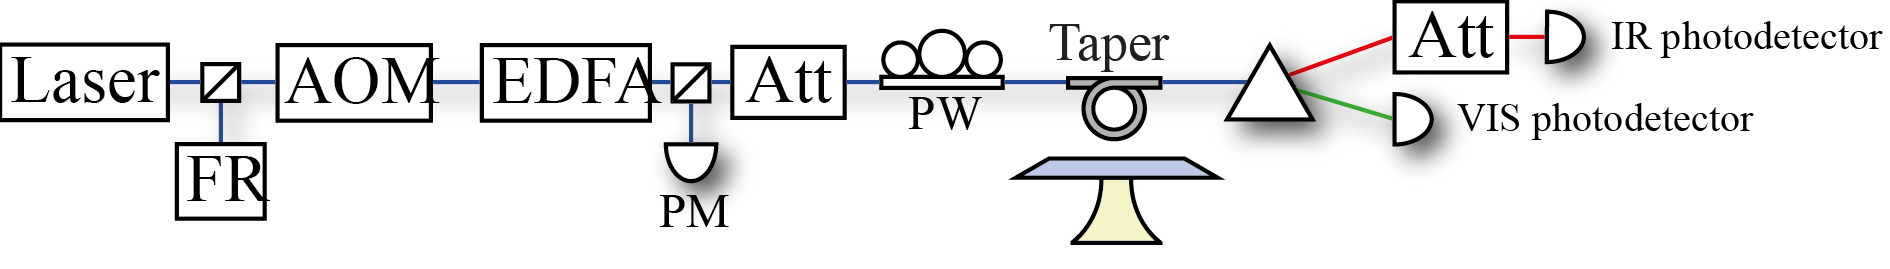
\includegraphics[width = 16 cm]{figuras/Dissertation_thg_setup.jpg}
    \caption{Experimental Setup: A infrared tunable Laser is modulated by a Acousto-optic Modulator (AOM) and amplified by a Erbium Doped Fiber Amplifier (EDFA) up to tens of watts. A Frequency Reference (FR) is used to precisely determine the frequency of the source, attenuator (att.) and paddle wheels are used to control the input power and polarization. The infrared part is splitted from the visible by a prism.}
    \label{fig:thg_setup}
\end{figure}

%in this paragraph I will talk about how to amplify the optical power
As seen in Chapter~\ref{chap:nonlin_pol}, to observe third order effects it is needed a power higher than the used in transmission experiment. To reach power high enough to the experiment a Erbium Doped Fiber Amplifier is applied, which amplifies the optical power to around $40$ dBm, to reach even higher power, the input wave is modulated in pulses with width of $400$~ns and duty cycle of $40$~$\mu$s using a Acousto-optic Modulator. 

The amplified power is monitored using a beam splitter. A fentosecond detector able to solve the pulse format enables to measured the power in function of time with the aid of a oscilloscope. The input power is controlled using a Attenuator, to keep the power measured by the IR photodetector at constant range another Attenuator is add to the circuit, the sum of the attenuation in both is keep constant.  

The experiment is done by sweep the frequency of the source and monitoring the power at the VIS photodetector. The result of the experiment is the power in visible band in function of the frequency of the source, as show in Fig.~\ref{fig:thg_broad_map}, each peak corresponds to a scenario wheres the condition to third harmonic generations, as sens in Chapter~\ref{chap:couple_mode}; this result was obtained as a preliminary result with the initial defective wafer. 
\begin{figure}[h]
    \centering
    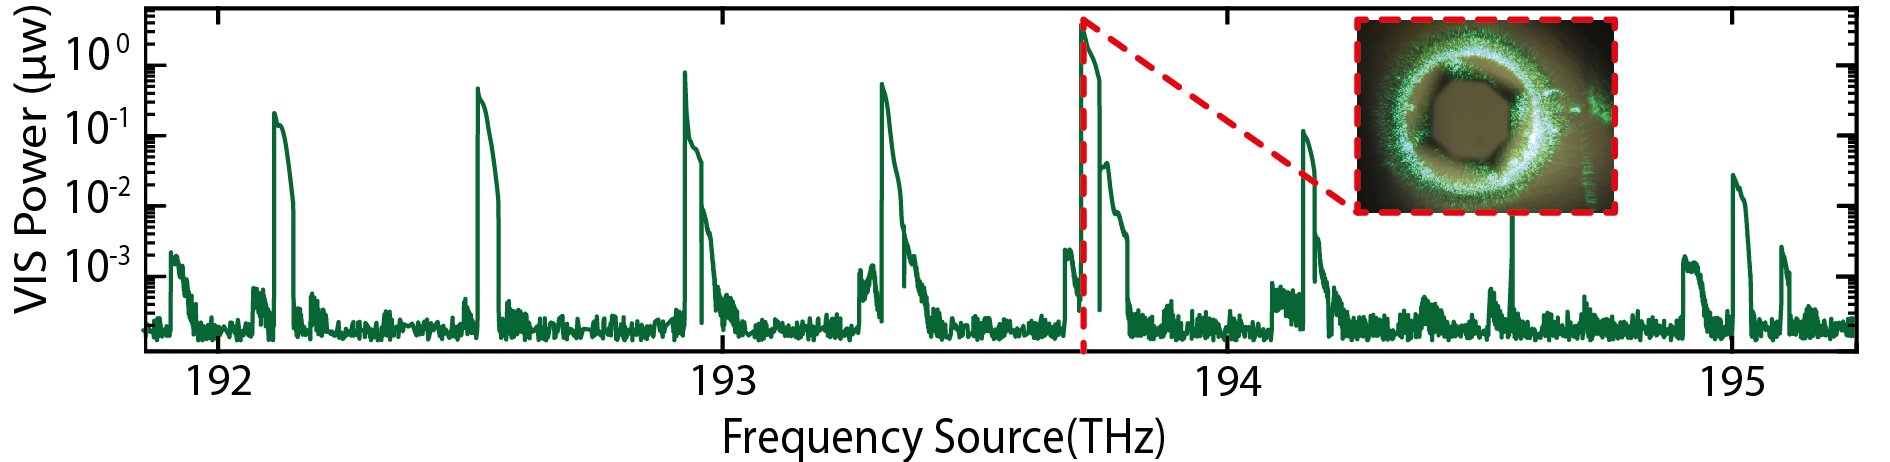
\includegraphics[width = 16cm]{figuras/Dissertation_thg_broad.jpg}
    \caption{Caption}
    \label{fig:thg_broad_map}
\end{figure}

The shape of the THG curves is significantly different of those predicted in the Fig.~\ref{fig:temporal_solution}, this is due to the interference between neighboring infrared modes. As the coupling between the cavity and the source must be high in in order to collect more TH, the amount of excited IR modes id high enough to produce a dirty transmission spectrum. 

Now we are interested in control the phase matching condition between the modes by change the phase detuning $\delta_omega$. To change the phase detuning we shall vary the sample temperature and due to a dynamics similar to the presented in the Eq~\ref{eq:termooptc_change}; however, with a external heat source instead of internal one; therefore the Eq~\ref{eq:pertubation_bistaliti_cavity} can by write as 
\begin{equation}
    \frac{\Delta\omega_\alpha}{\omega_\alpha} = \frac{d\text{n}_\alpha}{dt}\Delta T \rightarrow \Delta\delta_\omega = \left(\omega_3\frac{d\text{n}_3}{dt} - 3\omega_1\frac{d\text{n}_1}{dt}\right)\Delta T
    \label{eq:temperature_mode_variation}
\end{equation}
the frequency displacement due to the sample temperature is different for each band, leading to a variation in the initial phase detuning, even don't knowing the initial phase detuning $\delta_0$ it is possible to calculate the variation in the phase detuning in function of the temperature and compare the effect over the third harmonic generation. 

The experimental result can be quantitatively compared with the numerical solution of the Eq~\ref{eq:taxa_ir_broad} and Eq~\ref{eq:taxa_vis_broad} for different values of $\delta_\omega$. The result is presented in Fig.. This measurement was made using the piezo frequency control of the laser, preventing the infrared mode to interfere with the neighbors, another technique was to slight increase the diameter of the tapered fiber, in relation with the Fig.~\ref{fig:thg_broad_map}, leading to a decrease in the amount of visible power collected. Another important difference is the use of samples fabricated with lab grown wafer.

In order to produce a quantitative comparation we need to measured the parameters cited above.  

\section{Optical Characterization at Visible Band}

The main challenge in characterize the cavity in the visible band is the lack of a tunable visible laser, which could be used as described in the Sections~\ref{sec:optical_char}. As we do not have access to a visible tunable laser, we need to apply a different techniques, two to be precise. One technique use the transmitted light from a external source, slightly similar from the infrared characterization, the other one use the third harmonic internally generated. 

\subsection{Transmission Characterization}

This experiment is based on the Eq~\ref{eq:single_mode_transmission}, wheres the Detuning $\Delta_3$ (do not mistake with the phase detuning $\delta_\omega$) was defined $\Delta_3 = \omega_3 - \omega$. The source used was a visible green laser ($532$~nm) with fixed frequency; therefore, in order to compute the transmission spectrum we vary the resonance frequency $\omega_3$ by change the sample temperature, according with the Eq.~\ref{eq:temperature_mode_variation} we can write 
\begin{equation}
    \Delta_3 = \omega_3\frac{d\text{n}_3}{dT}\Delta T.
\end{equation}
To determine the $\Delta T$ an infrared mode was used as probe, the details of the procedure can be find in the Appendix~\ref{app:experiment}.

The Fig. shows the result of the experiment. An infrared mode was characterize using the same procedure, as shown in Fig~a, where we can calculate the losses, $\kappa_1^{(i)} = 940\pm 50$~MHz and $\kappa_1^{(e)} = 180 \pm 6$~MHz, them we compare with the typical characterization (as described in Chapter~\ref{chap:optical_cavity}), show in Fig.~, we have measured $\kappa_1^{(i)} = 910\pm 20$~MHz and $\kappa_1^{(e)} = 173 \pm 2$~MHz, which showed a good agreement between the methods.

The results for the visible mode is shown in the Fig~. It was possible to identify three different modes which was fitted with a variation of the Eq~\ref{eq:single_mode_transmission} to include the neighbors~\needcit. We have found the values
\begin{table}[h]
\centering
\begin{tabularx}{8cm}{c|c|c|c}
Modo & $\kappa_i$ (MHz) & $\kappa_e$ (MHz) & $Q_i$ ($10^5$) \\ 
\hline                               
1 &$700\pm200$&$12\pm2$&$9.0\pm2.0$\\
2 &$870\pm60$&$59\pm3$&$6.6\pm0.4$\\
3 &$950\pm90$&$37\pm2$&$6.1\pm0.5$
\end{tabularx}
\caption{1}
\end{table}

It is important to notice that the measured modes are out of band where we have measured third harmonic as the fundamental mode for this visible modes lies around the $1596$~nm, out of the EDFA band; however, this result bring us a strong feeling about the coupling rate between the visible modes and the source. The bus waveguide was designed for coupling infrared modes, which lead to a poor coupling for visible mode, as demonstrated in the numerical solution, Appendix~\ref{app:numerical_met}, the amount of visible light collected is strong dependent on the coupling, this result explain the low collected power presented in the Fig..

This technique characterize both $\kappa_3^{(i)}$ and $\kappa_3^{(e)}$, although it do not characterize a mode that we can measure third harmonic. The next technique use the generation of third harmonic to measures the losses, so, we necessary will be looking for a mode the interest band, in exchange, it will only be possible to measure the total loss. 

\subsection{Third Harmonic Generation Characterization}




\section{Modes Identification}
%Descrevo a comparação entre as medidas de dispersão e as simulações. Acredito que a parte de validação da simulação pode entrar como um apêndice. 

\section{THG Efficiency Mapping}
%Acho que não tem muito segredo nessa sessão. 